% Preamble and Setup
\documentclass[
    aspectratio=169,
    xcolor=svgnames,
]{beamer}
\graphicspath{{../../figures}}
\hypersetup{
    hidelinks,
}
\usepackage[
    overridenote,
    %hidenotes,
]{pdfpc}
\usepackage{minted}
\setminted{
    breaklines,
    autogobble,
    frame=lines,
    fontsize=\small,
}
\usepackage{multimedia}
\usepackage{multirow}

% Theming
\usetheme{Berlin}
\usecolortheme{whale}
\beamertemplatenavigationsymbolsempty
\setbeamercovered{transparent}
% Paragraph spacing (list environments are unaffected)
\setlength{\parskip}{0.5\baselineskip}
% To undo spacing before a list (may break pagination, but okay in Beamer):
%\vspace{-\parskip}

% Support skipping miniframes
\makeatletter
\let\beamer@writeslidentry@miniframeson=\beamer@writeslidentry
\def\beamer@writeslidentry@miniframesoff{%
  \expandafter\ifblank\expandafter{\beamer@framestartpage}{}{
    % removed \addtocontents commands
    \clearpage\beamer@notesactions%
  }
  \let\beamer@writeslidentry=\beamer@writeslidentry@miniframeson
}
\newcommand*{\skipminiframe}{\let\beamer@writeslidentry=\beamer@writeslidentry@miniframesoff}
\makeatother
% Show ToC at the beginning of each section
\AtBeginSection{
    \skipminiframe
    \begin{frame}{Table of Contents}
        \transuncover[direction=180, duration=0.25]
        \setlength{\parskip}{0pt}
        \tableofcontents[currentsection, hideothersubsections]
    \end{frame}
}

% Overlay-aware commands
\renewcommand<>{\sout}[1]{
  % Strikeout (strikethrough, crossout)
  \alt#2{\beameroriginal\sout{#1}}{#1}
}


% Presentation Content
\title{Sound Effect: Convolution Playback}
\subtitle{for EELE 468}
\author{Lucas Ritzdorf}
\institute{Montana State Unviersity}
\date{March 1, 2024}
\titlegraphic{
\includegraphics{msu-logo}}

\begin{document}

\maketitle

% Sections:
%   1. Sound Effect Overview
%   2. The algorithm (i.e. the math and/or signal flow graph)
%   3. Your Matlab code that implements the sound effect.
%   4. The Control Parameters you will be using
%   5. Sound Effect examples (before and after) using various control parameters that modify the audio with distinct audio differences.
\section{Overview}


\begin{frame}{System Overview}

    Operational modes:

    \pause
    \begin{itemize}[<+->]
        \item Capture an impulse response from the audio input

        \item Apply a corresponding effect to the live audio stream:
        \begin{itemize}[<.->]
            \item Convolve the captured impulse with the most recent stream sample
            \item Add the resulting convolved values to the output sample buffer
        \end{itemize}
    \end{itemize}

    \pause[\thebeamerpauses]
    Mode-switching is controlled via user input (e.g. ``push this button to record an impulse'')

\end{frame}

\section{Effect Algorithm}


\begin{frame}{Convolution Overview}

    It is easiest to regard convolution in time as an operation which creates copies of one signal wherever the other has peaks.

    \begin{columns}[t]

        \column{0.3\textwidth}
        \begin{figure}
            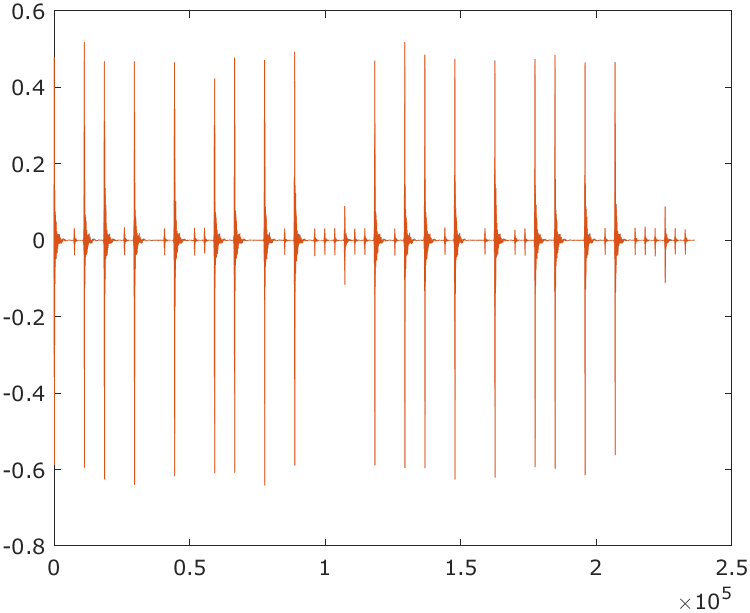
\includegraphics[height=0.4\textheight]{drum-wave}
            \caption{A drum sequence}
        \end{figure}

        \column{0.3\textwidth}
        \begin{figure}
            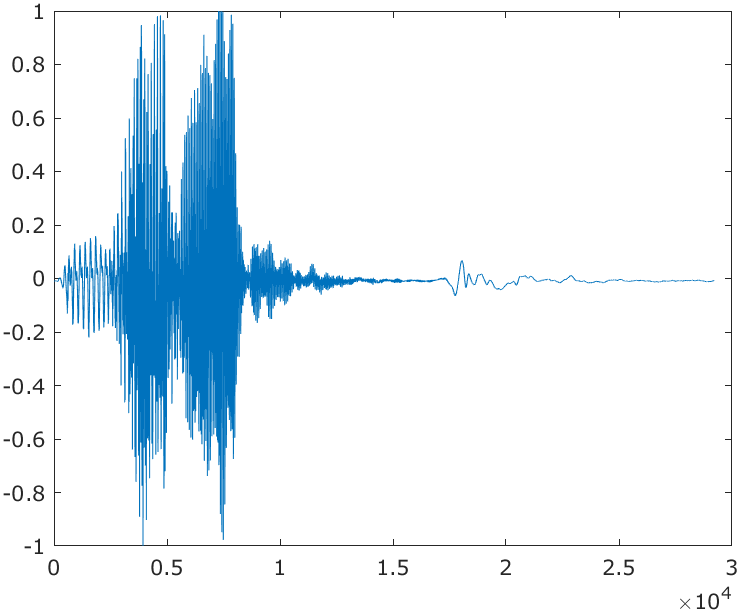
\includegraphics[height=0.4\textheight]{yop-wave}
            \caption{A ``Yop!''}
        \end{figure}

        \column{0.3\textwidth}
        \begin{figure}
            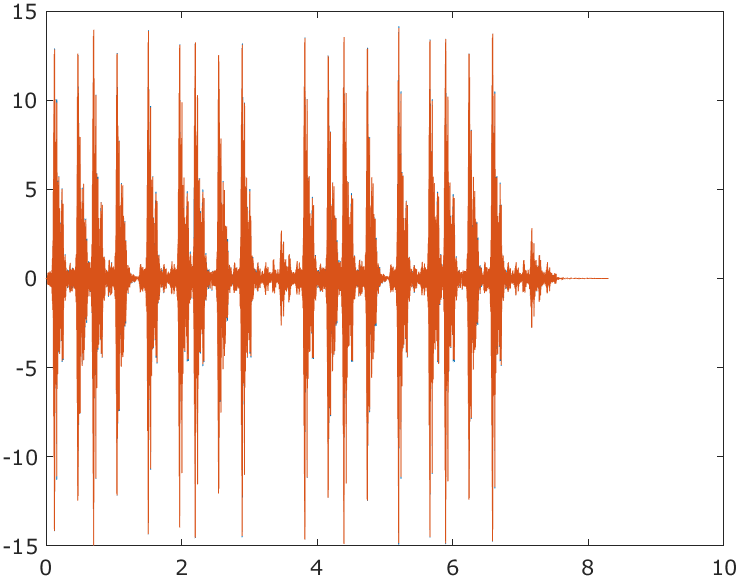
\includegraphics[height=0.4\textheight]{conv-wave}
            \caption{A drum sequence convolved with a ``Yop!''}
        \end{figure}

    \end{columns}

\end{frame}

\section{MATLAB Implementation}


\begin{frame}[fragile]{Loading Audio from Files}

    \texttt{uigetfile()} and \texttt{audioread()} allow us to import an audio file chosen by the user.

    \inputminted[firstline=8,lastline=15]{matlab}{../../effect/convolution_playback.m}

\end{frame}


\begin{frame}[fragile]{Recording Audio in Real Time}

    MATLAB also provides an \texttt{audiorecorder} object, which allows for real-time recording.

    \inputminted[firstline=26,lastline=34]{matlab}{../../effect/convolution_playback.m}

\end{frame}


\begin{frame}[fragile]{Signal Preprocessing}

    We ensure that the two signals have matching sampling frequencies and are in stereo.

    \inputminted[firstline=36,lastline=43]{matlab}{../../effect/convolution_playback.m}

\end{frame}


\begin{frame}[fragile]{Finally, Convolution!}

    At last, we can convolve the signals, making sure to incorporate wet/dry mixing.

    \inputminted[firstline=45,lastline=53,fontsize=\footnotesize]{matlab}{../../effect/convolution_playback.m}

\end{frame}

\section{Effect Parameters}


\begin{frame}{Parameters and Management}

    Managed by \alert<+-.(4)>{processor}: \\
    (i.e. memory-mapped registers, exposed to the HPS)

    \begin{itemize}[<+->]
        \item Wet/dry mix
        \item Recorded impulse duration (up to a limit set at compile time)
        \item User-interface controls (e.g. pre-recording delay)
    \end{itemize}

    Managed by \alert<+-.(2)>{user}:

    \begin{itemize}[<+->]
        \item Convolved impulse
    \end{itemize}

\end{frame}

\section{Audio Examples}


\begin{frame}{Inputs}

    The examples given here depend on several input sounds:

    \begin{table}
    \begin{tabular}{|l|l|l|}
        \textbf{Input} & \textbf{Impulse} & \textbf{Result} \\
        \hline

        \multirow{4}{*}{ \movie{\beamergotobutton{Acoustic guitar}}{../../effect/inputs/acoustic.wav} }
            & MIT Grassy Field & \movie{\beamergotobutton{Guitar in a Field}}{../../effect/examples/guitar_field.wav} \\
            & BIG HALL         & \movie{\beamergotobutton{Guitar in a Big Hall}}{../../effect/examples/guitar_bighall.wav} \\
            & Flangerspace     & \movie{\beamergotobutton{Guitar in a\dots{} Flangerspace?}}{../../effect/examples/guitar_flangerspace.wav} \\
            & Metallic Delay   & \movie{\beamergotobutton{Guitar but Metallic}}{../../effect/examples/guitar_metallic.wav} \\
        \hline

        \multirow{3}{*}{ \movie{\beamergotobutton{Drums from the Congo}}{../../effect/inputs/Congo Drummer.wav} }
            & BIG HALL         & \movie{\beamergotobutton{Drums in a Big Hall}}{../../effect/examples/drums_bighall.wav} \\
            & Metallic Delay   & \movie{\beamergotobutton{Drums but Metallic}}{../../effect/examples/drums_metallic.wav} \\
            & The ``Yop!''     & \movie{\beamergotobutton{Drums but ``Yop!''}}{../../effect/examples/drums_yop.wav} \\
        \hline

        \multirow{2}{*}{ \movie{\beamergotobutton{The ``Yop!''}}{../../effect/inputs/yop.wav} }
            & BIG HALL         & \movie{\beamergotobutton{Yop in a Big Hall}}{../../effect/examples/yop_bighall.wav} \\
            & Robotic Reverb   & \movie{\beamergotobutton{Yop with Robotic Reverb}}{../../effect/examples/yop_robotverb.wav} \\

    \end{tabular}
    \end{table}

\end{frame}


\end{document}
